\chapter{Tabla comparativa del set completo de moléculas}
\label{apend:pagina_tabla_intro_grande}

Para no hacer la tabla comparativa más grande de lo que ya es, se indican aquí los nombres de las moléculas junto con un identificador. Este identificador se usa a lo largo del documento en varias ocasiones para hacer referencia a estos nombres.

\begingroup
\renewcommand{\arraystretch}{1.5}

\begin{longtable}{cp{11cm}}
\caption{Tabla de índices con los nombres de las moléculas de la Tabla \ref{tabla:tabla_grande_apendice}}\\
    \hline
\textbf{Id} & \textbf{Nombre del compuesto} \\ \hline
\endfirsthead

\multicolumn{2}{c}%
{{\bfseries \tablename\ \thetable{} -- Continuación de la página anterior}} \\
\hline
 \textbf{Id} & \textbf{Nombre del compuesto} \\ \hline
\endhead

\hline \multicolumn{2}{r}{{Continúa en la siguiente página}} \\
\endfoot

\hline
\endlastfoot

1 & Methyl(triphenylphosphine)gold(I)  \\
%\hline
 2 & trans-Dibromobis(triphenylphosphine)palladium(II) \\
%\hline
 3 & Dichloro(1,5-cyclooctadiene)palladium(II) \\
%\hline
 4 & SK-CC 01A \\
%\hline
 5 & Bis[\textmu-chloro[5-hydroxy-2-[1-(hydroxyimino)ethyl]phenyl]palladium] \\
%\hline
 6 & (SP-4-3)-(3,5-Dichloro-2,4,6-trifluorophenyl)iodobis (triphenylarsine)palladium \\
%\hline


 7 & Palladium,(2,2\textquotesingle-bipyridine-\textit{k}N1,\textit{k}N1\textquotesingle)[(2,2-dimethyl-1,2-ethanediyl)-1,2-phenylene]fluoro(4-methylbenzenesulfonamidato-\textit{k}N)-, (OC-6-35)  \\
%\hline
 8 & Dibromo(1,2-dimethoxyethane)nickel(II) \\
%\hline
 9 & Bis(triphenylphosphine)ruthenium(II) dicarbonyl chloride \\
%\hline
 10 & Chloro(trimethylphosphine)gold(I) \\
%\hline
 11 & Chloro[tris(para-trifluoromethylphenyl)phosphine]gold(I) \\
%\hline
 12 & Chloro(dimethylsulfide)gold(I) \\
%\hline

 13 & Chloro(methyldiphenylphosphine)gold(I)  \\
%\hline
 14 & Chloro[diphenyl(o-tolyl)phosphine]gold(I) \\
%\hline
 15 & Chloro[(1,1\textquotesingle-biphenyl-2-yl)di-tert-butylphosphine]gold(I) \\
%\hline
 16 & (Acetonitrile)[(2-biphenyl)di-tert-butylphosphine] gold(I)hexafluoroantimonate \\
%\hline
 17 & Chloro[2-di-tert-butyl(2\textquotesingle,4\textquotesingle,6\textquotesingle-triisopropylbiphenyl)phosphine] gold(I) \\
%\hline
 18 & Chloro[2-dicyclohexyl(2\textquotesingle,4\textquotesingle,6\textquotesingle-trisopropylbiphenyl)phosphine]gold(I) \\
%\hline

 19 & BisPhePhos XD gold(I) chloride  \\
%\hline
 20 & Chloro[di(1-adamantyl)-2-dimethylaminophenylphosphine]gold(I) \\
%\hline
 21 & Dichloro(DPPE)digold(I) \\
%\hline
 22 & Dichloro[($\pm$)-BINAP]digold(I) \\
%\hline
 23 & Bis(chlorogold(I)) [1,1\textquotesingle-bis(diphenylphosphino)ferrocene] \\
%\hline
 24 & [(IMes)AuCl] \\
%\hline

 25 & [(IPr)AuCl]  \\
%\hline
 26 & IPrAuNTf2 \\
%\hline
 27 & DPPF \\
%\hline
 28 & Dicarbonylcyclopentadienyliodoiron(II) \\
%\hline
 29 & (OC-6-11\textquotesingle)-Bis[2,6-di(2-pyridinyl-\textit{k}N)phenyl-\textit{k}C]iron\\
 %\hline
30 & Chloro[5-methoxy-2-[1-[(4-methoxyphenyl)imino-\textit{k}N]ethyl]phenyl-\textit{k}C][(1,2,3,4,5-$\eta$)-1,2,3,4,5-pentamethyl-2,4-cyclopentadien-1-yl]iridium \\
%\hline
31 & Diiodo(pentamethylcyclopentadienyl)iridium(III) dimer
 \label{tabla:tabla_indices_apendice}
\end{longtable}

\endgroup




\begin{landscape}

% \small
\begin{longtable}{m{0.3cm}m{6.7cm}m{7.7cm}m{2.3cm}m{2.3cm}}
\caption{Tabla extendida para el set de datos de 30 moléculas. Contiene la cadena SMILES extraída de Sigma-Aldrich (SA), la cadena SMILES extraída de SciFinder (SF), y las imágenes de las respectivas bases de datos (SA y SF)}\\
\hline
 \textbf{Id} & \textbf{SMILES SA} & \textbf{SMILES SF} & \textbf{Imagen SA} & \textbf{Imagen SF} \\ \hline
\endfirsthead

\multicolumn{5}{c}%
{{\bfseries \tablename\ \thetable{} -- Continuación de la página anterior}} \\
\hline
\textbf{Id} & \textbf{SMILES SA} & \textbf{SMILES SF} & \textbf{Imagen SA} & \textbf{Imagen SF} \\ \hline
\endhead

\hline \multicolumn{5}{r}{{Continúa en la siguiente página}} \\
\endfoot

\hline
\endlastfoot

% Compuesto 2 del excel
 1 &
 C[Au].c1ccc(cc1)P(c2ccccc2) c3ccccc3 & 
 [Au+]([CH3-])[P](C=1C=CC=CC1) (C=2C=CC=CC2)C=3C=CC=CC3 & 
 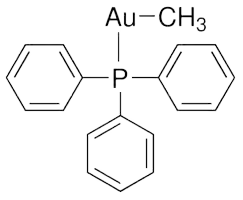
\includegraphics[width=2.2cm]{imagenes/sigmaAldrich/Methyl(triphenylphosphine)gold(I).png} & 
 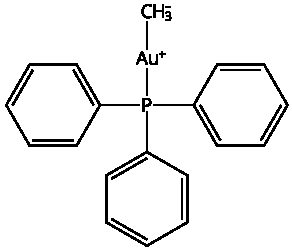
\includegraphics[width=2.2cm]{imagenes/sciFinder/pdf/Methyl(triphenylphosphine)gold(I).pdf} \\
%\midrule

% Compuesto 3 del excel
 2 &
 Br[Pd]Br.c1ccc(cc1) P(c2ccccc2)c3ccccc3.c4ccc(cc4) P(c5ccccc5)c6ccccc6 & 
 [Br-][Pd+2]([Br-])([P](C=1C= CC=CC1)(C=2C=CC=CC2) C=3C=CC=CC3)[P](C=4C=CC=CC4) (C=5C=CC= CC5)C=6C=CC=CC6 & 
 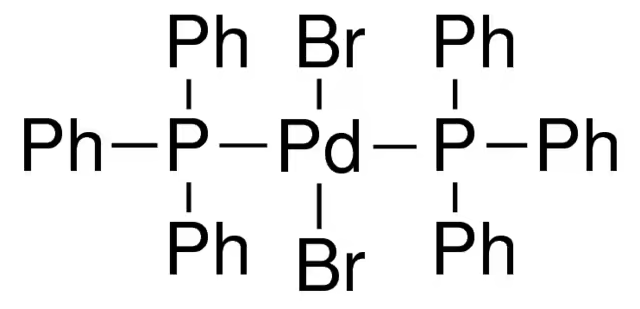
\includegraphics[width=2.2cm]{imagenes/sigmaAldrich/trans-Dibromobis(triphenylphosphine)palladium(II).png} & 
 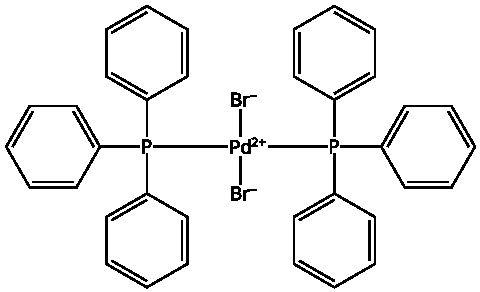
\includegraphics[width=2.2cm]{imagenes/sciFinder/pdf/trans-Dibromobis(triphenylphosphine)palladium(II).pdf} \\
%\midrule

% Compuesto 4 del excel
 3 &
 Cl[Pd]Cl.C1CC=CCCC=C1 & 
 [Cl-][Pd+2]123([Cl-]) [CH]=4CC[CH]3=[CH]2CC[CH]41 & 
 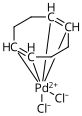
\includegraphics[width=2.2cm]{imagenes/sigmaAldrich/Dichloro(1,5-cyclooctadiene)palladium(II).png} & 
 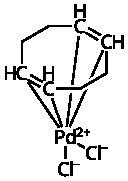
\includegraphics[width=2.2cm]{imagenes/sciFinder/pdf/Dichloro(1,5-cyclooctadiene)palladium(II).pdf} \\
%\midrule

% Compuesto 5 del excel
 4 &
 C1C[C@@H]2C[C@H]1CC2PC3C [C@@H]4CC[C@H]3C4.CN(C)c5ccccc5-c6ccccc6[Pd]Cl & 
 [Cl-][Pd+2]1([C-]=2C=CC=CC2C=3C =CC=CC3[N]1(C)C)[PH] (C4CC5CCC4C5)C6CC7CCC6C7 & 
 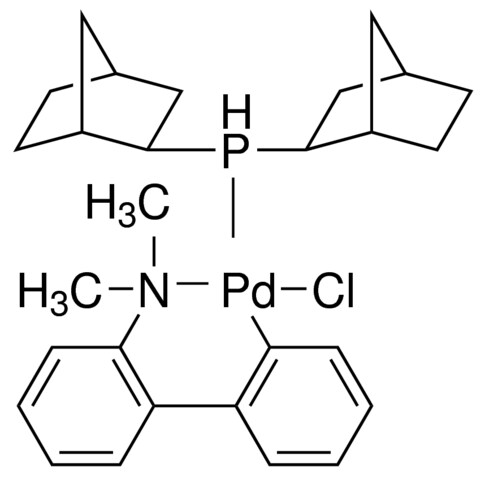
\includegraphics[width=2.1cm]{imagenes/sigmaAldrich/SK-CC 01A.jpeg} & 
 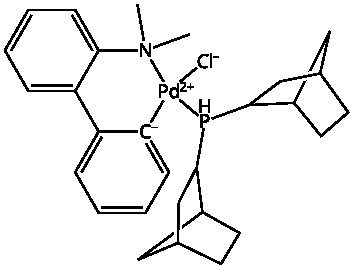
\includegraphics[width=2.2cm, height=2.1cm]{imagenes/sciFinder/pdf/SK-CC 01A.pdf} \\
%\midrule

% Compuesto 6 del excel
 5 &
 C\textbackslash C(=N/O)c1ccc(O)cc1[Pd]Cl .C\textbackslash C(=N/O)c2ccc(O)cc2[Pd]Cl & 
 OC=1C=CC=2C(=[N](O)[Pd+2]3 ([Cl-][Pd+2]4([Cl-]3)[C-]=5 C=C(O)C=CC5C(=[N]4O)C)[C-]2C1)C & 
 \includegraphics[width=2.2cm]{imagenes/sigmaAldrich/Bis[µ-chloro[5-hydroxy-2-[1-(hydroxyimino)ethyl]phenyl]palladium].jpeg} & 
 \includegraphics[width=2.2cm]{imagenes/sciFinder/pdf/Bis[µ-chloro[5-hydroxy-2-[1-(hydroxyimino)ethyl]phenyl]palladium].pdf} \\
%\midrule

\\ %Filas vacias para dar mas espacio entre el texto


% Compuesto 7 del excel
 6 &
 No se encontró el compuesto en Sigma-Aldrich & 
 FC=1C(Cl)=C(F)[C-](=C(F)C1Cl)[Pd+2] ([I-])([As](C=2C=CC=CC2)(C=3C=CC=C C3)C=4C=CC=CC4)[As](C=5C=CC=CC5) (C=6C=CC=CC6)C=7C=CC=CC7 & 
 & 
 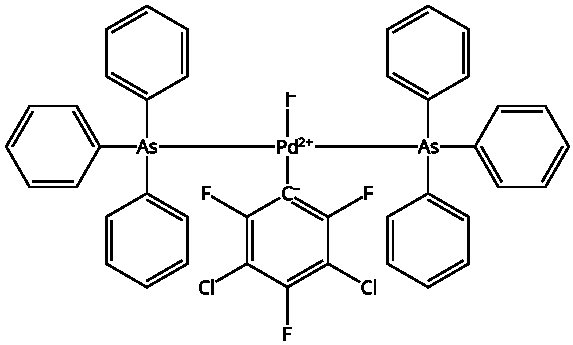
\includegraphics[width=2.5cm]{imagenes/sciFinder/pdf/(SP-4-3)-(3,5-Dichloro-2,4,6-trifluorophenyl)iodobis(triphenylarsine)palladium.pdf} \\
%\midrule

\\ %Filas vacias para dar mas espacio entre el texto

% Compuesto 8 del excel
 7 &
 No se encontró el compuesto en Sigma-Aldrich & 
 O=S(=O)([NH-][Pd+4]12([F-])([C-]=3C=CC=CC3C(C)(C)[CH2-]1) [N]=4C=CC=CC4C=5C=CC=C[N] 52)C6=CC=C(C=C6)C & 
 & 
 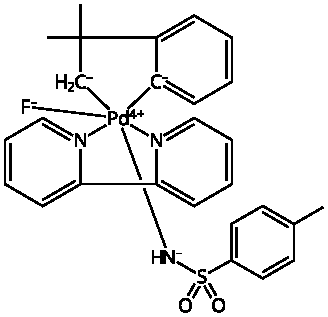
\includegraphics[width=2.2cm]{imagenes/sciFinder/pdf/Palladium, (2,2-bipyridine-κN1,κN1)[(2,2-dimethyl-1,2-ethanediyl)-1,2-phenylene]fluoro(4-methylbenzenesulfonamidato-κN)-, (OC-6-35).pdf} \\
%\midrule


% Compuesto 9 del excel
 8 &
 Br[Ni]Br.COCCOC & 
 [Br-][Ni+2]1([Br-])O(C)CCO1C & 
 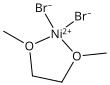
\includegraphics[width=2.2cm]{imagenes/sigmaAldrich/Nickel(II) bromide ethylene glycol dimethyl ether complex.png} & 
 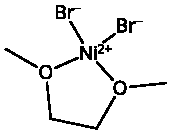
\includegraphics[width=2.2cm]{imagenes/sciFinder/pdf/Dibromo(1,2-dimethoxyethane)nickel(II).pdf} \\
%\midrule


% Compuesto 10 del excel
 9 &
 Cl[Ru](Cl)(C\#[O])(C\#[O])([PH](c1ccc cc1)(c2ccccc2)c3ccccc3)[PH](c4ccc cc4)(c5ccccc5)c6ccccc6 & 
 O\#C[Ru+2]([Cl-])([Cl-])(C\#O)([P](C=1C=CC=CC1) (C=2C=CC=CC2)C=3C=CC=CC3)[P] (C=4C=CC=CC4)(C=5C=CC=CC5) C=6C=CC=CC6 & 
 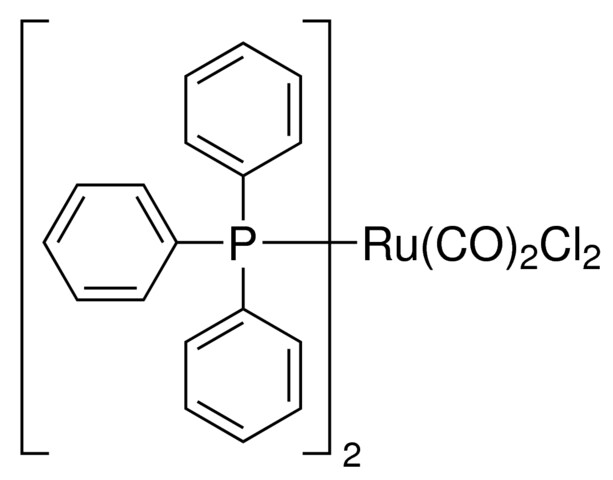
\includegraphics[width=2.2cm]{imagenes/sigmaAldrich/Bis(triphenylphosphine)ruthenium(II) dicarbonyl chloride.jpeg} & 
 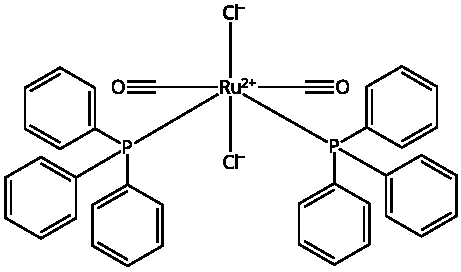
\includegraphics[width=2.2cm]{imagenes/sciFinder/pdf/Bis(triphenylphosphine)ruthenium(II) dicarbonyl chloride.pdf} \\
%\midrule

% Compuesto 11 del excel
 10 &
 Cl[Au].CP(C)C & 
 [Cl-][Au+][P](C)(C)C & 
 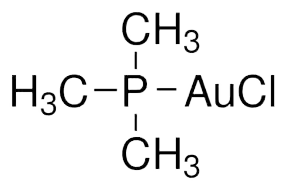
\includegraphics[width=2.2cm]{imagenes/sigmaAldrich/Chloro(trimethylphosphine)gold(I).png} & 
 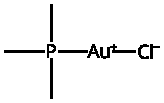
\includegraphics[width=2.2cm]{imagenes/sciFinder/pdf/Chloro(trimethylphosphine)gold(I).pdf} \\
%\midrule


% Compuesto 12 del excel
 11 &
 Cl[Au].FC(F)(F)c1ccc(cc1)P(c2ccc (cc2)C(F)(F)F)c3ccc(cc3)C(F)(F)F & 
 FC(F)(F)C1=CC=C(C=C1)[P] ([Au+][Cl-])(C2=CC=C(C=C2)C(F) (F)F)C3=CC=C(C=C3)C(F)(F)F & 
 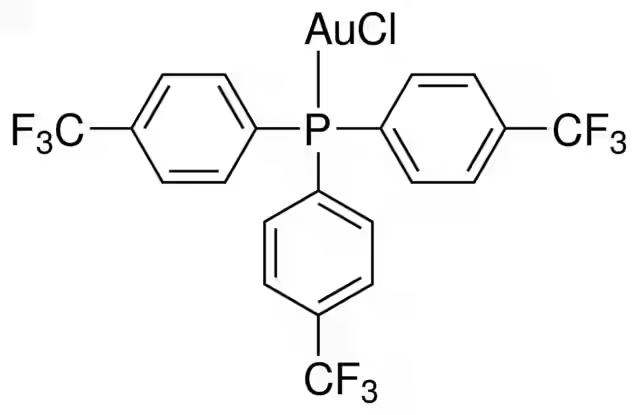
\includegraphics[width=2.2cm]{imagenes/sigmaAldrich/Chloro[tris(para-trifluoromethylphenyl)phosphine]gold(I).png} & 
 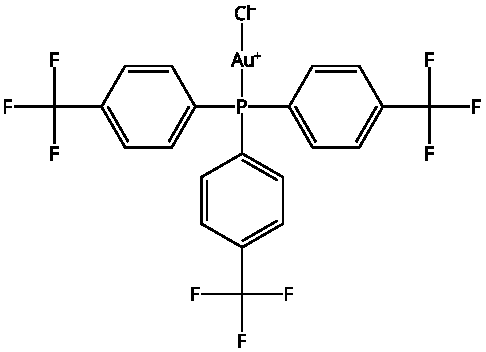
\includegraphics[width=2.2cm]{imagenes/sciFinder/pdf/Chloro[tris(para-trifluoromethylphenyl)phosphine]gold(I).pdf} \\
%\midrule



% Compuesto 13 del excel
 12 &
 Cl[Au].CSC & 
 [Cl-][Au+][S](C)C & 
 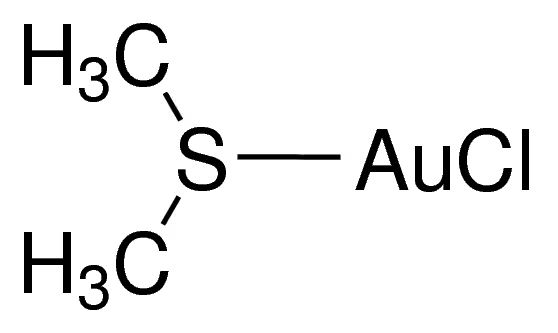
\includegraphics[width=2.2cm]{imagenes/sigmaAldrich/Chloro(dimethylsulfide)gold(I).png} & 
 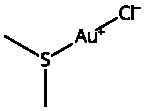
\includegraphics[width=2.2cm]{imagenes/sciFinder/pdf/Chloro(dimethylsulfide)gold(I).pdf} \\
%\midrule



% Compuesto 14 del excel
 13 &
 Cl[Au].CP(c1ccccc1)c2ccccc2 & 
 [Cl-][Au+][P](C=1C=CC=CC1) (C=2C=CC=CC2)C & 
 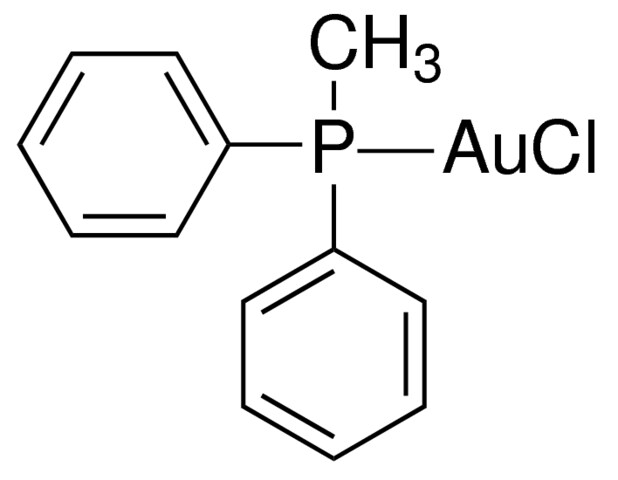
\includegraphics[width=2.1cm, height=1.5cm]{imagenes/sigmaAldrich/Chloro(methyldiphenylphosphine)gold(I).jpeg} & 
 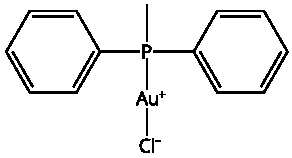
\includegraphics[width=2.2cm]{imagenes/sciFinder/pdf/Chloro(methyldiphenylphosphine)gold(I).pdf} \\
%\midrule




% Compuesto 15 del excel
 14 &
 Cl[Au].Cc1ccccc1P(c2ccccc2)c3ccccc3 & 
 [Cl-][Au+][P](C=1C=CC=CC1) (C=2C=CC=CC2)C=3C=CC=CC3C & 
 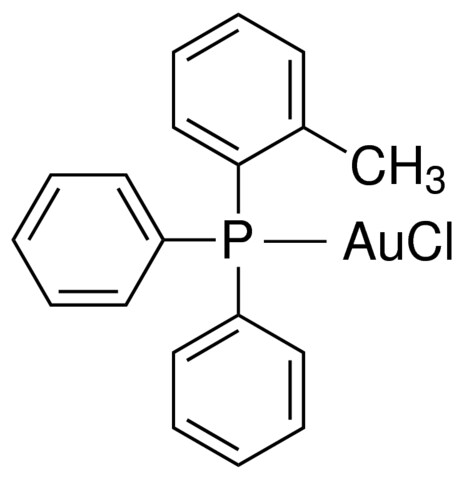
\includegraphics[width=2.2cm]{imagenes/sigmaAldrich/Chloro[diphenyl(o-tolyl)phosphine]gold(I).jpeg} & 
 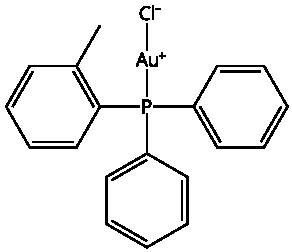
\includegraphics[width=2.2cm]{imagenes/sciFinder/pdf/Chloro[diphenyl(o-tolyl)phosphine]gold(I).pdf} \\
%\midrule


% Compuesto 16 del excel
 15 &
 Cl[Au].CC(C)(C)P(c1ccccc1-c2ccccc2)C(C)(C)C & 
 [Cl-][Au+][P](C=1C=CC=CC1C=2C =CC=CC2)(C(C)(C)C)C(C)(C)C & 
 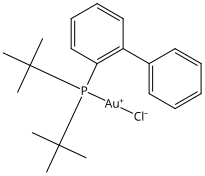
\includegraphics[width=2.2cm]{imagenes/sigmaAldrich/Chloro[(1,1-biphenyl-2-yl)di-tert-butylphosphine]gold(I).png} & 
 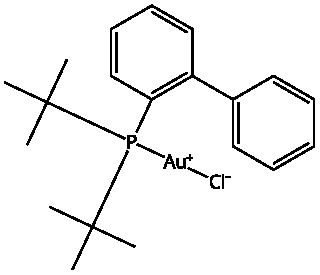
\includegraphics[width=2.2cm]{imagenes/sciFinder/pdf/Chloro[(1,1-biphenyl-2-yl)di-tert-butylphosphine]gold(I).pdf} \\
%\midrule



% Compuesto 17 del excel
 16 &
 [Au+].CC\#N.F[Sb-](F)(F)(F)(F)F. CC(C)(C)P(c1ccccc1-c2ccccc2)C(C)(C)C & 
 [F-][Sb+5]([F-])([F-])([F-])([F-])[F-]. C(\#[N][Au+][P](C=1C=CC=CC1C= 2C=CC=CC2)(C(C)(C)C)C(C)(C)C)C & 
 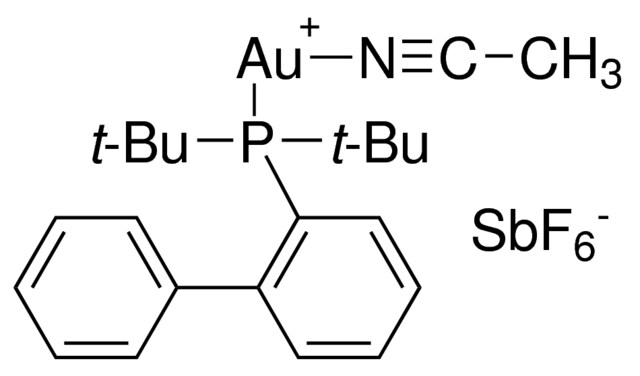
\includegraphics[width=2.2cm]{imagenes/sigmaAldrich/(Acetonitrile)[(2-biphenyl)di-tert-butylphosphine]gold(I) hexafluoroantimonate.jpeg} & 
 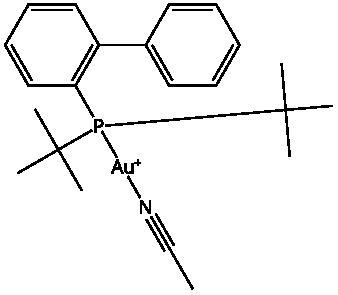
\includegraphics[width=2.2cm]{imagenes/sciFinder/pdf/(Acetonitrile)[(2-biphenyl)di-tert-butylphosphine]gold(I) hexafluoroantimonate [1compuesto].pdf} \\
  &  &  &  &
 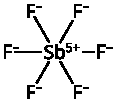
\includegraphics[width=2.2cm]{imagenes/sciFinder/pdf/(Acetonitrile)[(2-biphenyl)di-tert-butylphosphine]gold(I) hexafluoroantimonate [2compuesto].pdf} \\
%\midrule



% Compuesto 18 del excel
 17 &
 CC(C)c1cc(C(C)C)c(c(c1)C(C)C)-c2 ccccc2[PH]([Au]Cl)(C(C)(C)C)C(C)(C)C & 
 [Cl-][Au+][P](C=1C=CC=CC1C=2C (=CC(=CC2C(C)C)C(C)C)C(C)C)(C(C) (C)C)C(C)(C)C & 
 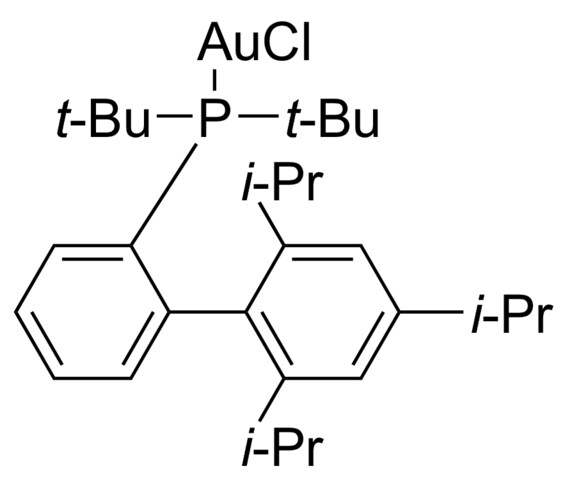
\includegraphics[width=2.2cm]{imagenes/sigmaAldrich/Chloro[2-di-tert-butyl(2,4,6-triisopropylbiphenyl)phosphine] gold(I).jpeg} & 
 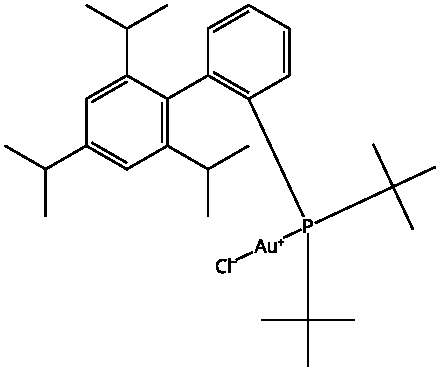
\includegraphics[width=2.3cm]{imagenes/sciFinder/pdf/Chloro[2-di-tert-butyl(2,4,6-triisopropylbiphenyl)phosphine] gold(I).pdf} \\
%\midrule



% Compuesto 19 del excel
 18 &
 Cl[Au].CC(C)c1cc(C(C)C)c(c(c1)C(C) C)-c2ccccc2P(C3CCCCC3)C4CCCCC4 & 
 [Cl-][Au+][P](C=1C=CC=CC1C=2C (=CC(=CC2C(C)C)C(C)C)C(C)C)(C3C CCCC3)C4CCCCC4 & 
 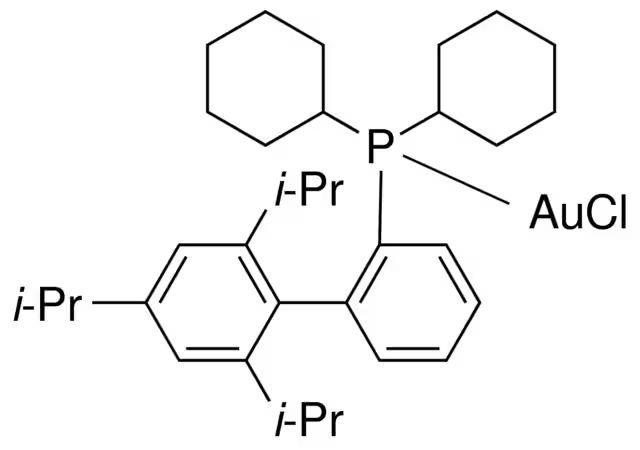
\includegraphics[width=2.2cm]{imagenes/sigmaAldrich/Chloro[2-dicyclohexyl(2,4,6-trisopropylbiphenyl)phosphine]gold(I).png} & 
 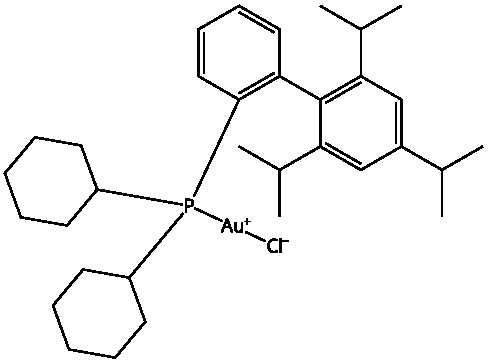
\includegraphics[width=2.2cm]{imagenes/sciFinder/pdf/Chloro[2-dicyclohexyl(2,4,6-trisopropylbiphenyl)phosphine]gold(I).pdf} \\
%\midrule

\\ %Filas vacias para dar mas espacio entre el texto

% Compuesto 20 del excel
 19 &
 CC(C)OC(C=CC=C1OC(C)C)=C1C2 =CC(P(C3CCCCC3)C4=CC(C5=C(O C(C)C)C=CC=C5OC(C)C)=CC=C4) =CC=C2.[Au]Cl & 
 [Cl-][Au+][P](C=1C=CC=CC1C2=C(OC(C) C)C=CC=C2OC(C)C)(C=3C=CC=CC3C4 =C(OC(C)C)C=CC=C4OC(C)C)C5CCCCC5 & 
 \includegraphics[width=2.2cm]{imagenes/sigmaAldrich/pdf/BisPhePhos XD gold(I) chloride.pdf} & 
 \includegraphics[width=2.2cm]{imagenes/sciFinder/pdf/BisPhePhos XD gold(I) chloride.pdf} \\
%\midrule



% Compuesto 21 del excel
 20 &
 Cl[Au].CN(C)c1ccccc1P(C23C C4CC(CC(C4)C2)C3)C56CC7CC(C C(C7)C5)C6 & 
 [Cl-][Au+][P](C=1C=CC=CC1N (C)C)(C23CC4CC(CC(C4)C2)C3) C56CC7CC(CC(C7)C5)C6 & 
 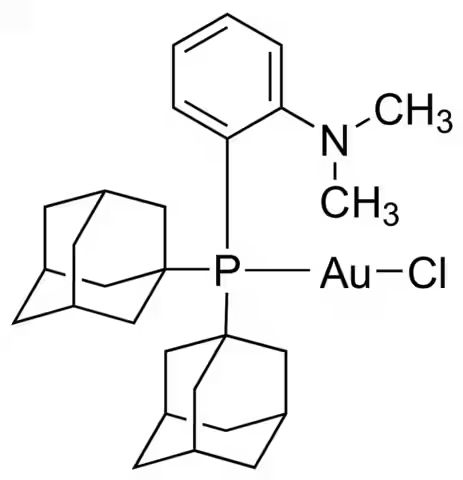
\includegraphics[width=2.2cm]{imagenes/sigmaAldrich/Chloro[di(1-adamantyl)-2-dimethylaminophenylphosphine]gold(I).png} & 
 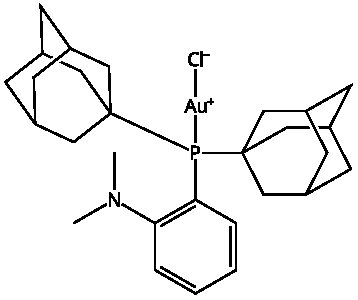
\includegraphics[width=2.2cm]{imagenes/sciFinder/pdf/Chloro[di(1-adamantyl)-2-dimethylaminophenylphosphine]gold(I).pdf} \\
%\midrule





% Compuesto 22 del excel
 21 &
 Cl[Au].Cl[Au].C(CP(c1ccccc1) c2ccccc2)P(c3ccccc3)c4ccccc4 & 
 [Cl-][Au+][P](C=1C=CC=CC1) (C=2C=CC=CC2)CC[P]([Au+][Cl-]) (C=3C=CC=CC3)C=4C=CC=CC4 & 
 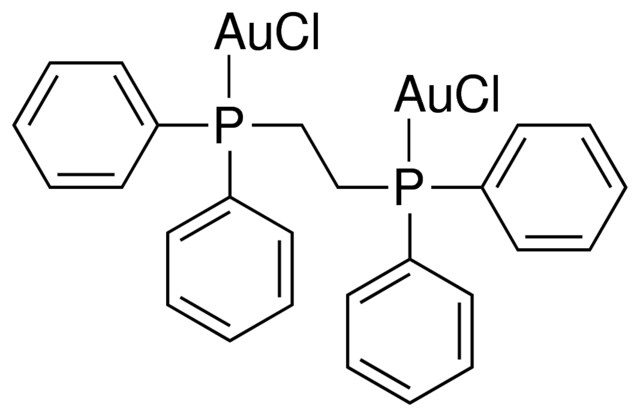
\includegraphics[width=2.2cm]{imagenes/sigmaAldrich/Dichloro(DPPE)digold(I).jpeg} & 
 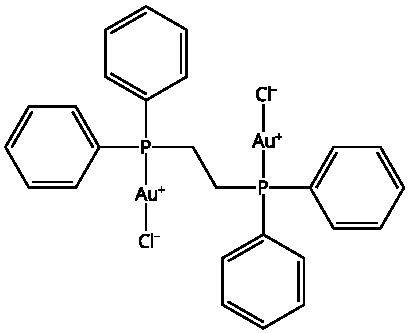
\includegraphics[width=2.2cm]{imagenes/sciFinder/pdf/Dichloro(DPPE)digold(I).pdf} \\
%\midrule


% Compuesto 23 del excel
 22 &
 Cl[Au].Cl[Au].P(C1=CC=CC=C1)(C2 =C(C3=C(C=CC4=C3C=CC=C4)P (C5=CC=CC=C5)C6=CC=CC=C6)C7 =C(C=CC=C7)C=C2)C8=CC=CC=C8 & 
 [Cl-][Au+][P](C=1C=CC=CC1)(C=2C =CC=CC2)C3=CC=C4C=CC=CC4=C3 C=5C=6C=CC=CC6C=CC5[P]([Au+] [Cl-])(C=7C=CC=CC7)C=8C=CC=CC8 & 
 
\includegraphics[width=2.2cm]{imagenes/sigmaAldrich/Dichloro[(±)−BINAP]digold(I).png} & 
 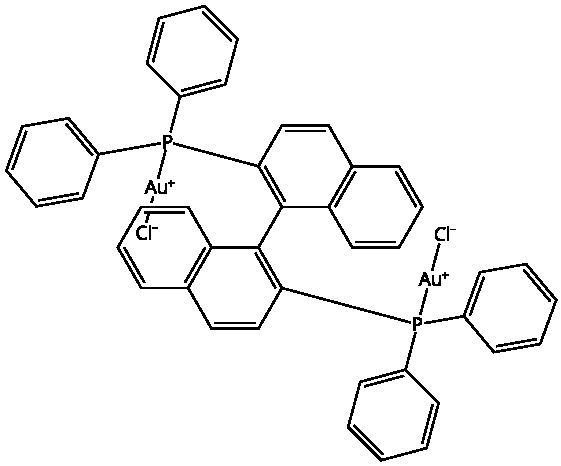
\includegraphics[width=2.2cm]{imagenes/sciFinder/pdf/Dichloro[(±)−BINAP]digold(I).pdf} \\
%\midrule


% Compuesto 24 del excel
 23 &
 [Fe].Cl[Au].Cl[Au].[CH]1[CH] [CH][C]([CH]1)P(c2ccccc2)c3 ccccc3.[CH]4[CH][CH][C]([CH]4) P(c5ccccc5)c6ccccc6 & 
 [Cl-][Au+][P](C=1C=CC=CC1)(C=2C=CC =CC2)[C-]34[CH]5=[CH]6[CH]7=[CH]3[Fe+2] 6789\%10\%1154[CH]=\%12[CH]\%11=[CH]\%10 [C-]9([CH]\%128)[P]([Au+][Cl-])(C=\%13 C=CC=CC\%13)C=\%14C=CC=CC\%14 & 
 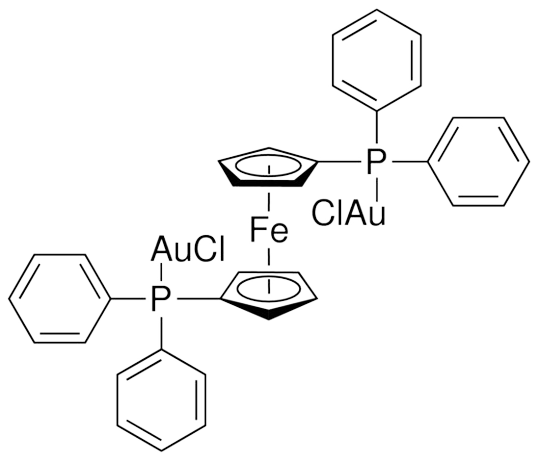
\includegraphics[width=2.5cm]{imagenes/sigmaAldrich/pdf/Bis(chlorogold(I)) [1,1-bis(diphenylphosphino)ferrocene.png} & 
 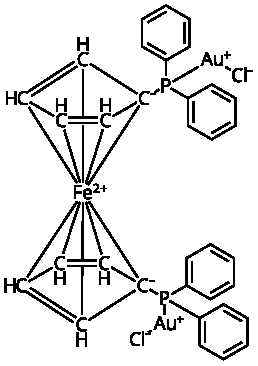
\includegraphics[width=2.2cm]{imagenes/sciFinder/pdf/Bis(chlorogold(I)) [1,1-bis(diphenylphosphino)ferrocene].pdf} \\
%\midrule


% Compuesto 25 del excel
 24 &
 Cl[Au].Cc1cc(C)c(N2[C]N(C=C2) c3c(C)cc(C)cc3C)c(C)c1 & 
 Cl[Au]=C1N(C=CN1C=2C(=CC(=CC2 C)C)C)C=3C(=CC(=CC3C)C)C & 
 \includegraphics[width=2.2cm]{imagenes/sigmaAldrich/pdf/[(IMes)AuCl].pdf} & 
 \includegraphics[width=2.2cm]{imagenes/sciFinder/pdf/[(IMes)AuCl].pdf} \\
%\midrule


% Compuesto 26 del excel
 25 &
 CC(C)c1cccc(C(C)C)c1N2C=CN(C2 [Au]Cl)c3c(cccc3C(C)C)C(C)C & 
 Cl[Au]=C1N(C=CN1C=2C(=CC=CC2C (C)C)C(C)C)C=3C(=CC=CC3C(C)C)C(C)C & 
 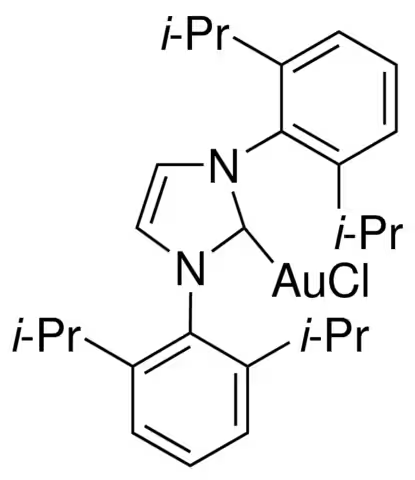
\includegraphics[width=2.2cm]{imagenes/sigmaAldrich/[(IPr)AuCl].png} & 
 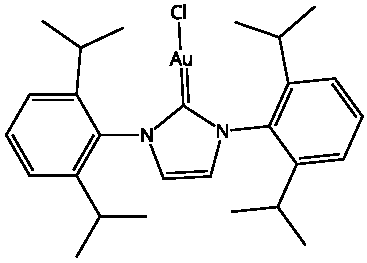
\includegraphics[width=2.2cm]{imagenes/sciFinder/pdf/[(IPr)AuCl].pdf} \\
%\midrule

% Compuesto 27 del excel
 26 &
 CC(C)c1cccc(C(C)C)c1N2C=CN(C2= [Au]N(S(=O)(=O)C(F)(F)F)S(=O) (=O)C(F)(F)F)c3c(cccc3C(C)C)C(C)C & 
 O=S(=O)(N([Au]=C1N(C=CN1C=2C(= CC=CC2C(C)C)C(C)C)C=3C(=CC=CC3C (C)C)C(C)C)S(=O)(=O)C(F)(F)F)C(F)(F)F & 
 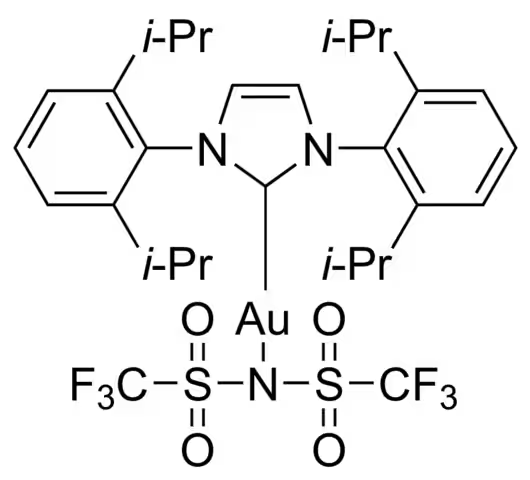
\includegraphics[width=2.1cm]{imagenes/sigmaAldrich/IPrAuNTf2.png} & 
 \includegraphics[width=2.2cm]{imagenes/sciFinder/pdf/IPrAuNTf2.pdf} \\
%\midrule

% Compuesto 29 del excel
 27 &
 [Fe].[CH]1[CH][CH][C]([CH]1)P (c2ccccc2)c3ccccc3.[CH]4[CH][CH] [C]([CH]4)P(c5ccccc5)c6ccccc6 & 
 C=1C=CC(=CC1)P(C=2C=CC=CC2) [C-]34[CH]5=[CH]6[CH]7=[CH]3[Fe+2] 6789\%10\%1154[CH]=\%12[CH]\%11= [CH]\%10[C-]9(P(C=\%13C=CC=CC\%13) C=\%14C=CC=CC\%14)[CH]\%128 & 
 \includegraphics[width=2.2cm]{imagenes/sigmaAldrich/DPPF.png} & 
 \includegraphics[width=2.2cm]{imagenes/sciFinder/pdf/DPPF.pdf} \\
%\midrule

% Compuesto 30 del excel
 28 &
 [Fe]I.[C-]\#[O+].[C-]\#[O+]. [CH]1[CH][CH][CH][CH]1 & 
 O\#C[Fe+2]1234([I-])(C\#O)[CH]= 5[CH]4=[CH]3[CH-]2[CH]51 & 
 \includegraphics[width=2.2cm]{imagenes/sigmaAldrich/Dicarbonylcyclopentadienyliodoiron(II).png} & 
 \includegraphics[width=2.2cm]{imagenes/sciFinder/pdf/Dicarbonylcyclopentadienyliodoiron(II).pdf} \\
%\midrule

% Compuesto 31 del excel
 29 &
 No se encontró el compuesto en Sigma-Aldrich & 
 C=1C=C[N]2=C(C1)C3=CC=CC=4C=5C= CC=C[N]5[Fe+2]672([C-]34)[C-]=8C(=CC=CC8C=9C=CC=C [N]96)C=\%10C=CC=C[N]\%107 & 
 & 
 \includegraphics[width=2.2cm]{imagenes/sciFinder/pdf/(OC-6-11)-Bis[2,6-di(2-pyridinyl-κN)phenyl-κC]iron.pdf}\\
%\midrule

% Compuesto 32 del excel
 30 &
 [CH]1[CH][CH][CH][CH]1.COc2ccc (cc2)\textbackslash N=C(/C)c3ccc(OC)cc3[Ir]Cl & 
 [Cl-][Ir+3]12345([C-]6=CC(OC)=C C=C6C(=[N]1C=7C=CC(OC)=C C7)C)C=8(C)C5(C)=C4(C)[C-]3(C)C82C & 
 \includegraphics[width=2.2cm]{imagenes/sigmaAldrich/iridio_solo.png} & 
 \includegraphics[width=2.2cm]{imagenes/sciFinder/iridio_solo.png}\\
%\midrule

% Compuesto 33 del excel
 31 &
 I[Ir]I.I[Ir]I.C[C]1[C](C)[C](C)[C](C) [C]1C.C[C]2[C](C)[C](C)[C](C)[C]2C & 
 [I-][Ir+3]12345([I-][Ir+3]6789([I-])([I-]1)C=\%10(C)C9(C)=C8(C)[C-]7(C)C \%106C)C=\%11(C)C5(C)=C4(C) [C-]3(C)C\%112C & 
 \includegraphics[width=2.2cm]{imagenes/sigmaAldrich/iridio_doble.png} & 
 \includegraphics[width=2.2cm]{imagenes/sciFinder/iridio_doble.png}
% \hline
\label{tabla:tabla_grande_apendice}

\end{longtable}

\end{landscape}


